\subsection{Secondary transfer to ds006780}
The secondary transfer evaluated \DsRunCount{} selected runs on
\DsSubjectCount{} participants, producing \DsPredictionCount{} predictions.
At 200 HBN training subjects, the rich-statistics head had a mean Pearson
difference of \DsSecondaryDelta{} from the baseline, with 95\% interval
[\DsSecondaryCILow{},\,\DsSecondaryCIHigh{}]. At 800 training subjects, the
difference was \DsPrimaryDelta{} and all \DsPrimaryWins{} seed differences
were positive, but its interval also included zero:
[\DsPrimaryCILow{},\,\DsPrimaryCIHigh{}].

The 800-subject interval width was \DsPrimaryCIWidth{}, exceeding the planned
maximum of \DsPrecisionMaxWidth{}. Thus the precision gate failed. The interval
both leaves the direction of the population advantage uncertain and is wider
than intended; this analysis does not establish stable superiority.
Table~\ref{tab:ds006780-summary} and Figure~\ref{fig:ds006780} report the results.

\begin{table}[tbp]
  \centering
  \small
  \caption{Secondary ds006780 transfer. Pearson and seed SD summarize ten
  training runs. Paired differences and joint intervals compare the rich head
  with the baseline at the same training size.}
  \label{tab:ds006780-summary}
  \begin{tabular}{llrrrr}
\toprule
Training $n$ & Head & Pearson & Seed SD & $\Delta r$ & 95\% interval \\
\midrule
200 & Mean-pooled linear & 0.2650 & 0.0141 & -- & -- \\
200 & Rich-statistics residual & 0.2577 & 0.0168 & -0.0073 & [-0.0861, 0.0721] \\
800 & Mean-pooled linear & 0.3255 & 0.0091 & -- & -- \\
800 & Rich-statistics residual & 0.3543 & 0.0107 & 0.0287 & [-0.0349, 0.0922] \\
\midrule
\multicolumn{6}{l}{Precision gate: failed; observed width 0.1272, threshold 0.0600.} \\
\bottomrule
\end{tabular}

\end{table}

\begin{figure}[tbp]
  \centering
  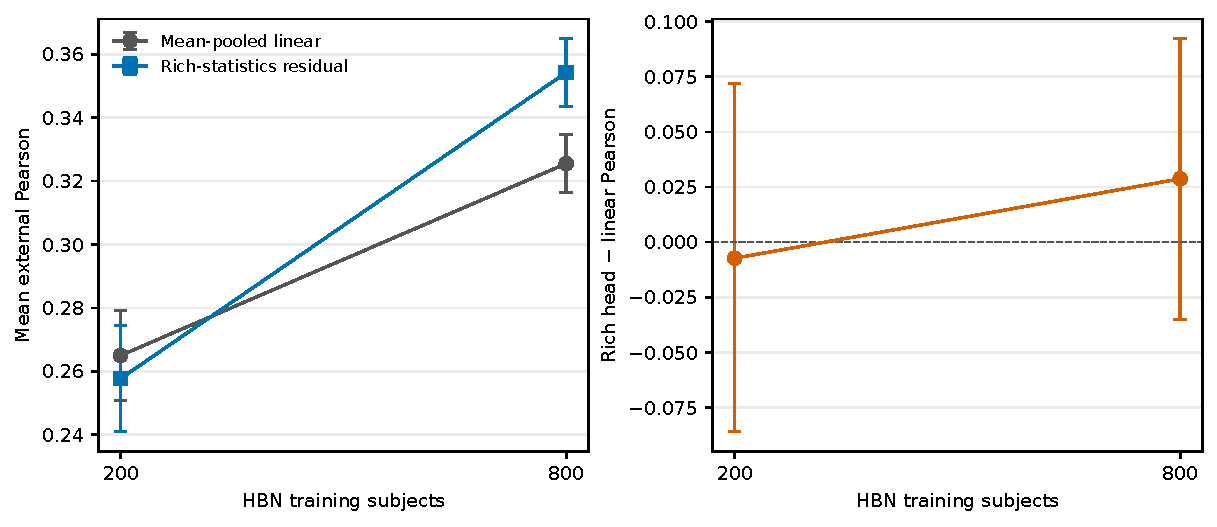
\includegraphics[width=0.95\linewidth]{../results/extensions/ds006780_external_v5/ds006780_external.pdf}
  \caption{Secondary ds006780 results. Left: Pearson correlations with standard
  deviations across seeds. Right: paired differences with intervals that also
  resample participants. Both intervals include zero.}
  \label{fig:ds006780}
\end{figure}
